\section{Method}

Segments of the data running both L1 (Livingston, Louisiana) and H1 (Hanford, Washington) without inconsistently large noise were used within the S6 run, which occurred from July 2009 through October 2010. The time-series data was filtered with a bandpass filter between 100 and 300 Hz to eliminate low- and high-frequency noise. Figures~\ref{figa} and~\ref{figb} illustrate a sample signal before and after this filtering, respectively, showing this effect. This filtering leaves a filter response, which appears predominantly at the start of the studied segment, figure~\ref{impulse} shows the filter response from an impulse signal, which can be seen to last a few minutes, therefore, the first 3 minutes of every segment were cut off before carrying on with the analysis.

\begin{figure}[htb]
\begin{center}
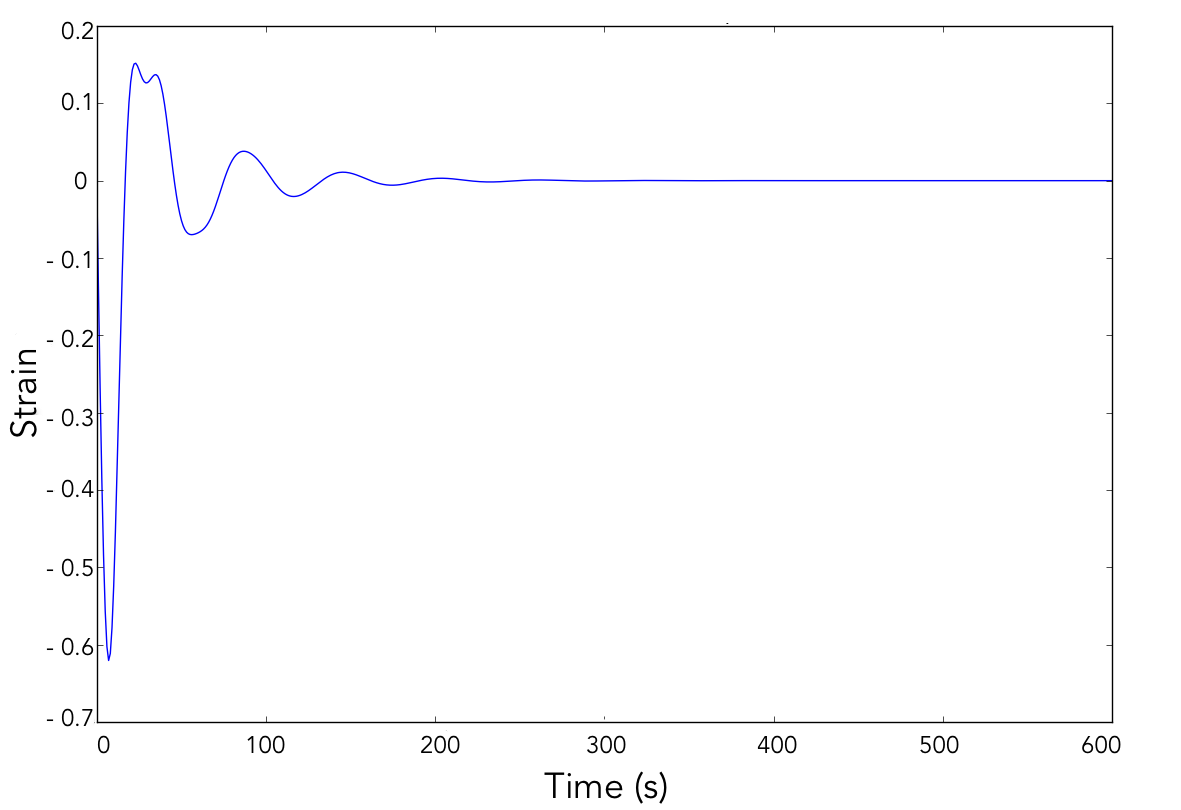
\includegraphics[width=0.9\textwidth]{impulse}
\caption{Filter response for an impulse signal}
\label{impulse}
\end{center}
\end{figure}

\par{}
The coordinates of the Sun were used to set the time-delay between the two detectors. These coordinates change, however, and therefore the time-delay should also change accordingly so that the detectors keep pointing at the Sun. Figure~\ref{tdt} shows the sinusoidal change of the time-delay for a little over a day ($10^{5}$ seconds). The largest allowable change of coordinates, with regards to the sensitivity of the detector, was chosen such that the change in time-delay is always smaller than $0.05 \over \omega$ where $\omega$ is the angular frequency, from that it follows that the maximum allowable change in time-delay is 0.0000265. Figure~\ref{ddt} shows a comparison of different durations to update the coordinates at, to test the change in time-delay, and illustrates why choosing 30-second segments is thus a legitimate choice. 
\begin{figure}[htb]
\begin{center}
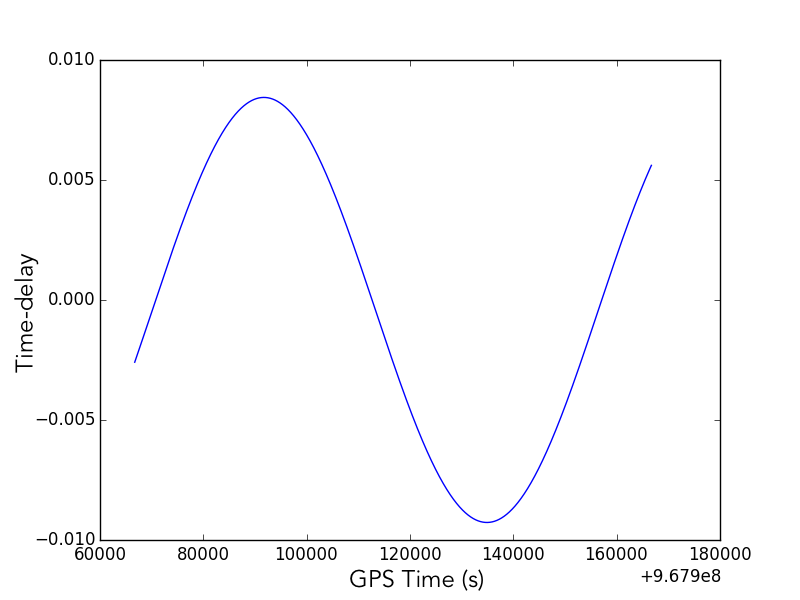
\includegraphics[width=\textwidth]{t_dt}
\caption{Time-delay over approx. 28 hours ($10^{5}$ seconds)}
\label{tdt}
\end{center}
\end{figure}
\par{} 
The same data with 100 different time-delays pointing where the position of the Sun was at different times (10, 20, 30, etc. minutes before) were used for the background signal. This might potentially eliminate false-positives as the background now has the same periodicity as the Sun.

\begin{figure}[htb]
\begin{center}
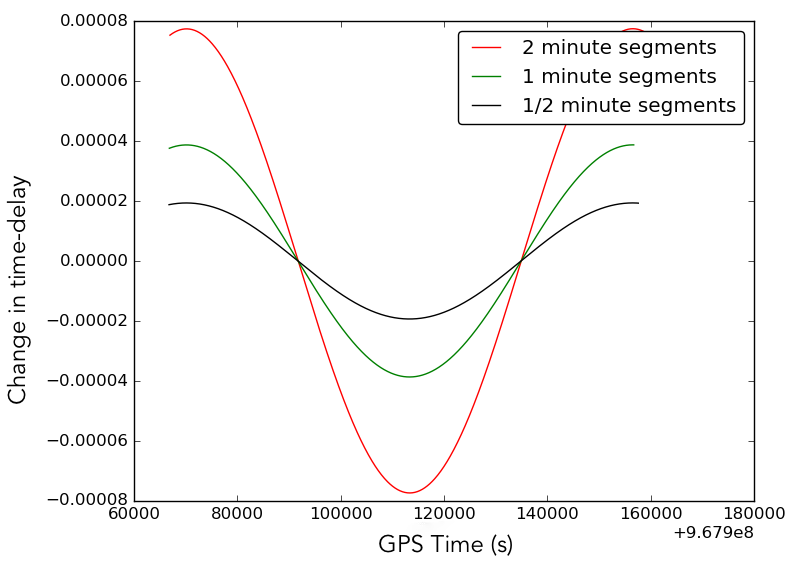
\includegraphics[width=0.9\textwidth]{ddt}
\caption{Change of time-delay over a day for several segments. The selected segment duration needs to be less than 0.000026 to keep the detectors in sync. 30 seconds was chosen as the 'coordinates update time'.}
\label{ddt}
\end{center}
\end{figure}\par{}
% talk about figure
\par{}
The dot product of the 30-second segments for the two detectors were then taken to cross-correlate their signals, for both the Solar and background signals, to compare them and look for GW detection.
